\documentclass{article}
\usepackage[utf8]{inputenc}
\usepackage[T1]{fontenc}
\setlength{\parindent}{0cm}
\usepackage[margin=1in]{geometry}
\usepackage{tgpagella} %font
\usepackage{graphicx} %figures
\graphicspath{ {Figures/} } %figures
\usepackage{hyperref} %make hyperlinks
\usepackage{fancyhdr} %to get headers
\pagestyle{fancy} %to get headers

\title{Simstock QGIS Plugin docs}
\author{shyam.amrith.14 }
\date{June 2022}

\begin{document}

\begin{titlepage}
\begin{center}
\Huge
\textbf{Simstock QGIS Plugin}
\vspace{5mm}

\huge
\textbf{Documentation}

\vspace{2cm}
\large
The Bartlett School of Environment, Energy and Resources, UCL \\
\vspace{1mm}
June -- September 2022
\end{center}
\vspace{2cm}
\tableofcontents
\end{titlepage}
\clearpage

\section{Installation, setup and testing}
\subsection{Supported QGIS versions}
The plugin has been tested on a range of QGIS versions, on both Windows and Mac operating systems. The supported versions of QGIS are any LTR (long-term release) between QGIS LTR 3.10 and the latest QGIS LTR 3.22. \\

The non-LTR versions are likely to work too, however sometimes the Python versions and associated packages in these versions differ from the LTR versions. %For example QGIS 3.10.3 does not work as it does not have pandas installed.

\subsection{Installation}
\label{section:installation}
\begin{enumerate}
    \item Download and extract the zip folder containing the Simstock QGIS plugin. This should return a folder named \texttt{simstock\_qgis} as well as some files for testing. \label{step:zip}
    
    \item Launch QGIS. Navigate to \textbf{Settings $\rightarrow$ User Profiles $\rightarrow$ Open Active Profile Folder} from the top bar (see below).
    \begin{figure}[h!]
        \centering
        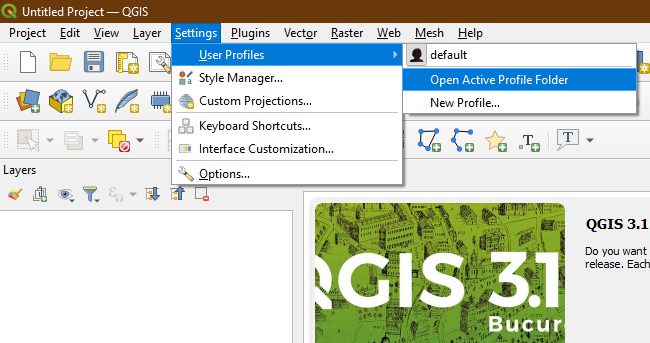
\includegraphics[width=12cm]{profile_folder.png}
        \label{fig:profile_folder}
    \end{figure}
    \item The previous step will open a file browser showing the QGIS profile folder. Using this file browser, open the folder named `\textbf{python}'. Next, open the folder named `\textbf{plugins}' if it exists. If not, create a new folder named `\textbf{plugins}' (note this must be all in lowercase), and then open it.
    
    \item Copy the entire extracted \texttt{simstock\_qgis} folder from step~\ref{step:zip} into the `plugins' folder (Note: copy the entire folder -- not just the contents).
    
    \item Restart QGIS. Once it has reloaded, navigate to \textbf{Plugins $\rightarrow$ Manage and Install Plugins} (see below).
    \begin{figure}[h!]
        \centering
        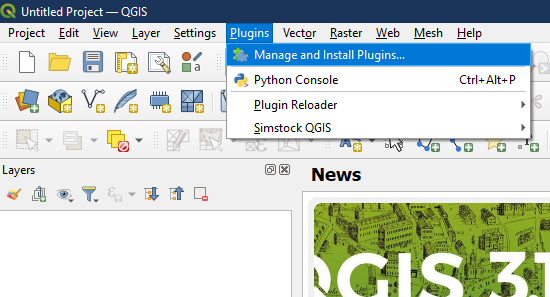
\includegraphics[width=12cm]{manage-plugins.png}
        \label{fig:manage_plugins}
    \end{figure}
    \clearpage
    
    \item Select `\textbf{Settings}' on the left panel and tick the box which says `\textbf{Show also experimental plugins}' (see below).
    \begin{figure}[h!]
        \centering
        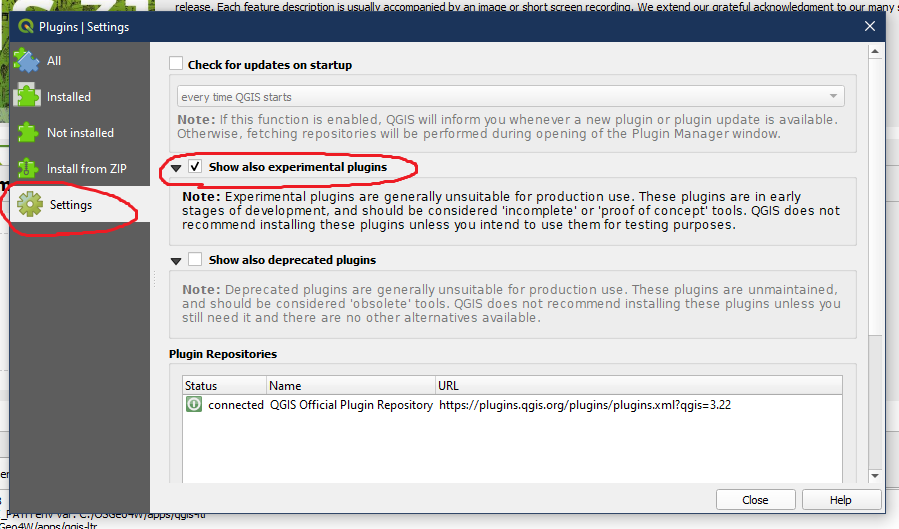
\includegraphics[width=14cm]{show_experimental.png}
        \label{fig:show_exp}
    \end{figure}
    
    \item Select `\textbf{All}' on the left panel and search for `\textbf{simstock}'. The plugin should now show up, and you can \textbf{tick the box} to install it. If the plugin is not listed, you may need to restart QGIS and repeat this step.
    \begin{figure}[h!]
        \centering
        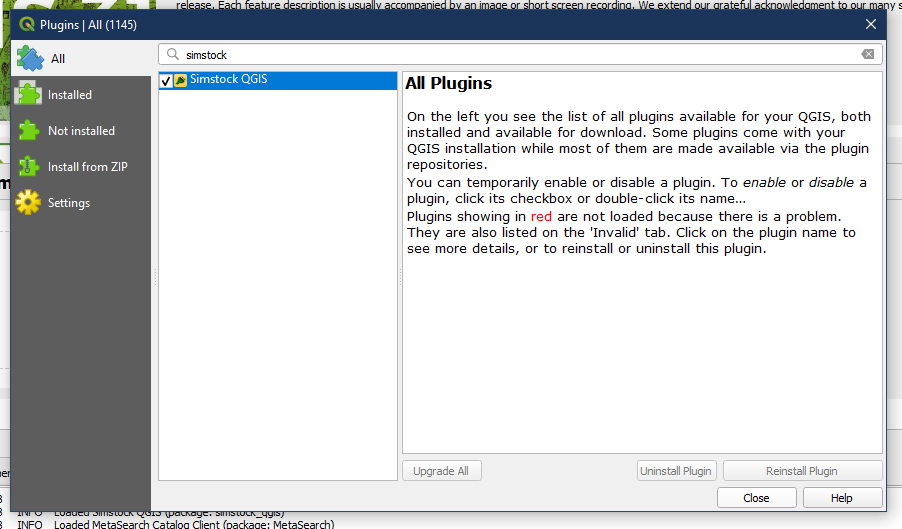
\includegraphics[width=14cm]{tick-simstock.png}
        \label{fig:tick_simstock}
    \end{figure}
    
    \item Also search for `Plugin Reloader' and tick the box when it shows up.
    
    \item After ticking the boxes, you will need to restart QGIS.
    
    \item If the Simstock QGIS plugin has successfully been installed, you should be able to see it listed under the `Plugins' list as well as a new icon on the toolbar (see below).
    \begin{figure}[h!]
        \centering
        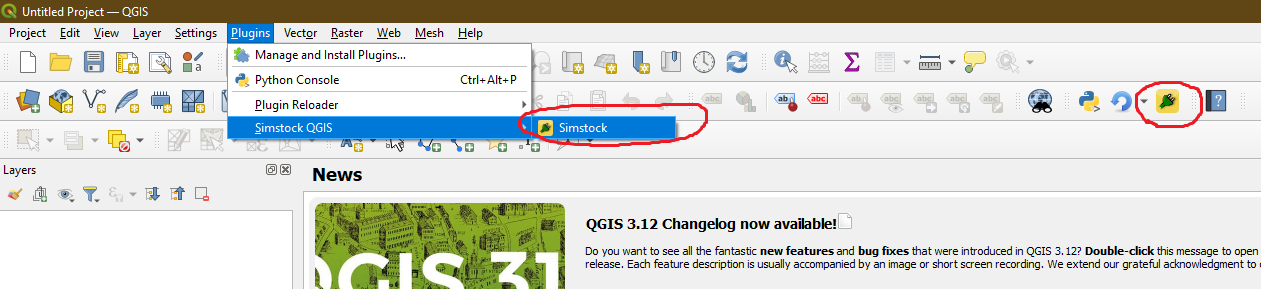
\includegraphics[width=16cm]{installed.png}
        \label{fig:installed}
    \end{figure}
    
    \item The plugin will now need to be tested -- see the next section for information.
\end{enumerate}

\subsection{Initial setup}
Before running anything, make sure that the QGIS Python Console is open as there will be outputs here that will be useful to read. It should open automatically when the plugin is launched, but if not, you can do this by clicking \textbf{Plugins $\rightarrow$ Python Console} in the top bar of QGIS. \\

When the plugin is launched, you will see an `initial setup' button. This will run checks to verify that all the dependencies are working as expected. \\

Click the `initial setup' button and watch the Python console for any errors. If any of the steps fail, they should be reported here. If all checks passed, a green success message should show up in the QGIS console. The plugin should now be fully functioning -- though you may need to restart QGIS for a final time.

%\iffalse
\subsection{Test on an example project}
\begin{enumerate}
    \item Locate the \texttt{testing.gpkg} project which was included in the zip file.
    \item Open the file by dragging it into the QGIS window. If you are unable to do this, you can also open it by navigating to Layer $\rightarrow$ Add Layer $\rightarrow$ Add Vector Layer in the top bar. You can then select the geopackage file here. Once opened, you should now see a layer called `testing'; a small area of polygons representing a few houses.
    \item Launch the Simstock plugin, and set your current working directory (cwd). Once you have selected a directory, click the green tick button. This is the location where all project files (including simulation results) will be stored. This should also add some database layers to the QGIS session.
    \item Next, make sure the testing layer is selected, and then click `Run'. This should generate a number of EnergyPlus idf files and simulate them. A new results layer will be added to the QGIS session. The idf files and simulation results can be found in the \texttt{idf\_files} directory within your cwd.
\end{enumerate}
\clearpage
%\fi

%\iffalse
\clearpage
\section{Using the plugin}
\subsection{Important notes}
There are some important things to note when using the plugin:
\begin{itemize}
    \item \textbf{Python Console}: When using the plugin, always have the Python console open. This will output information about what the plugin is doing. It should open by default when the plugin is launched, but if not, you can do this by clicking Plugins $\rightarrow$ Python Console in the top bar of QGIS.
    \item \textbf{Python Errors}: If an error occurs, a yellow notification appears in QGIS. The Python error can be viewed by clicking `Stack Trace'. This should give information about what is causing the error.
    \item \textbf{Plugin Reloader}: Make sure the Plugin Reloader is installed (see Section~\ref{section:installation}). If the Simstock plugin stops functioning correctly, reload it using the plugin reloader.
\end{itemize}

\subsection{The interface}
\begin{figure}[h!]
    \centering
    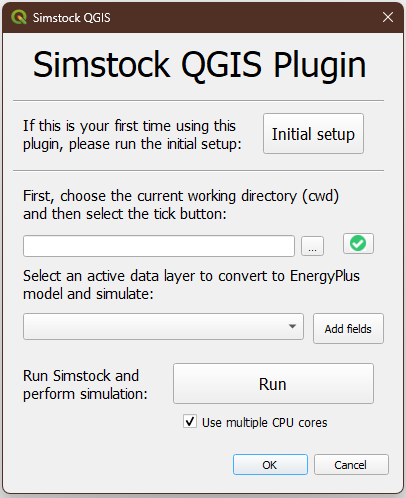
\includegraphics[width=8cm]{Figures/plugin_win11.png}
    \caption{The Simstock QGIS plugin UI}
    \label{fig:pluginui}
\end{figure}

\subsection{Input data}
Before the plugin is run, the input data must be prepared in such a way that Simstock can process it. \\

\textbf{Geometry} \\
The geometry (i.e. buildings footprints) must exist as a Vector Layer. There are no requirements about where this geometry is sourced from; it can be hand-drawn or acquired from a digital source. \\ %The plugin retrieves the geometry directly from the selected layer's feature geometries using the built-in QGIS Python API.

\textbf{Attribute table fields} \\
The input data for each polygon is specified via the QGIS attribute table. Simstock expects certain fields to exist here. These fields can be added to the Vector Layer by selecting the layer in the drop-down menu and clicking on the \textbf{Add Fields} button. This will add the following fields to the layer: %TODO: missing fields will cause mysterious errors
\begin{itemize}
    \item `\textbf{UID}' -- {Unique identifier} [string]
    \begin{itemize}
        \item The UIDs for each polygon are automatically generated by the plugin when the `Add Fields' button is pressed. The UIDs should NOT be changed. An ID that is unique to each polygon.% This is used by Simstock to name and identify zones and objects in the EnergyPlus model which belong to the given polygon. It is also used to retrieve the simulation results.
    \end{itemize}
    \item `\textbf{height}' -- {Building height (m)} [float]
    \begin{itemize}
        \item Expressed in metres.
    \end{itemize}
    \item `\textbf{shading}' [boolean string]
    \begin{itemize}
        \item FALSE -- Building is included in the energy modelling.
        \item TRUE -- Building is treated as a shading block. In this case, the only other attributes required for the given polygon are the UID and building height.
    \end{itemize}
    \item `\textbf{wwr}' -- {Window-to-wall/glazing ratio} (\%) [float]
    \begin{itemize}
        \item The ratio between the surface area of the window to the surface area of the wall for the building. Expressed as a percentage value between 0-100.
    \end{itemize}
    \item `\textbf{nofloors}' -- {Number of floors} [integer]
    \begin{itemize}
        \item Number of floors in the building. Determines how many thermal zones are stacked vertically within the EnergyPlus model for the given polygon.
    \end{itemize}
    \item `\textbf{construction}' [string]
    \begin{itemize}
        \item Used to select a construction preset from the database - explained further in Section~\ref{section:database}.
    \end{itemize}
    \item `\textbf{ventilation\_rate}' [float]
    \begin{itemize}
        \item Specifies the ventilation rate in `air changes per hour' (ACH). %($m^3s^{-1}\mathrm{person}^{-1}$).
        Applies to every zone in the building.
    \end{itemize}
    \item `\textbf{overhang\_depth}' -- {Shading overhang depth (m)} [float]
    \begin{itemize}
        \item Allows a shading overhang to be added to each window. If left blank or at `0' value, no overhangs are created. If a float value is specified, an overhang will be added to every window of the polygon with a depth of the specified amount in metres (m).
    \end{itemize}
\end{itemize}
\vspace{5mm}
After these fields have been added to the layer, they need to be filled out (except for the UID). \\

\textbf{Mixed-use} \\
After creating and filling out these fields, more optional fields can be created to specify the use on each floor (e.g. residential, commercial etc.). To do this, make sure the `\texttt{nofloors}' has been entered for every non-shading polygon, then click `Add Fields' again. This will add a new  `\texttt{FLOOR\_X:~use}' field for every floor. The options for these fields are: `Dwell', `Commercial' and `Workshop'. To understand what effect these choices have, see Section~\ref{section:mixeduse}. \\

This summarises the minimum input data required to run the plugin from start to finish. It is possible to specify much more detail via the database (see Section~\ref{section:database}), however if this step is omitted then the plugin will simply use the default database settings.


\subsection{Setting the current working directory (cwd)}
\label{section:cwd}
\textbf{What the cwd is} \\
The current working directory (cwd) is the folder where the project is setup and stored. This means that you can export the entire Simstock setup by sharing the cwd folder with another user. The following files will be output to the cwd:
\begin{itemize}
    \item The project-specific database files (covered in Section~\ref{section:database})
    \item The generated EnergyPlus \texttt{.idf} files
    \item The EnergyPlus simulation results
\end{itemize}
\textbf{How to set the cwd} \\
To set the cwd, browse to the desired path using the selector box and then select the green tick button. \\

The project database file will be called \texttt{Simstock-Database.gpkg}:
\begin{itemize}
    \item If this file does not exist in the cwd, it is created from defaults and saved here.
    \item If this file already exists in the cwd, it is loaded.
\end{itemize}

\subsection{Database}
\label{section:database}
Section~\ref{section:cwd} discussed how the database file is managed. This section will cover what the database is and how it can be viewed/edited. \\

\textbf{What it contains} \\
After the cwd has been set, a number of layers will be loaded into the QGIS project. Each layer corresponds to a different category of data required to generate the EnergyPlus models:
\begin{itemize}
    \item Fabric: Materials %x4
    \item Fabric: Constructions (arranges the materials)
    \item Schedules
    \item Loads: People
    \item Loads: Lighting
    \item Loads: Electrical equipment
    \item Heating + Cooling on/off toggle (explained in Section~\ref{section:heatingcoolingtoggle})
\end{itemize}

\subsubsection{Interacting with the database}
\textbf{Viewing} \\
Right-click on one of the database layers and click "Open Attribute Table". This will display the database in Table View -- see Figure~\ref{fig:db1}. Each row represents an individual element and the columns represent the fields of the element. A more intuitive way to view this is to select ``Form View'' at the bottom-right of the window -- see Figure~\ref{fig:db2}. \\

\begin{figure}[h!]
    \centering
    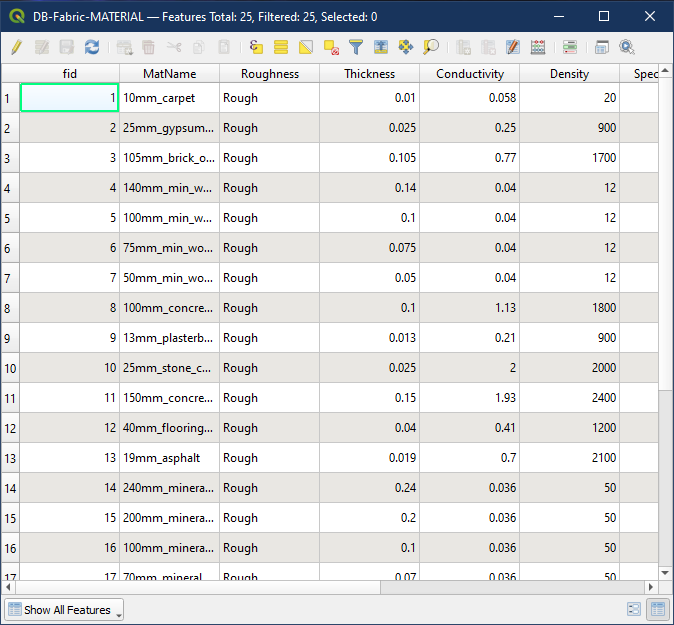
\includegraphics[width=10cm]{Figures/databaselayer1.png}
    \caption{The "\texttt{MATERIAL}" database layer, in Table View.}
    \label{fig:db1}
\end{figure}
\begin{figure}[h!]
    \centering
    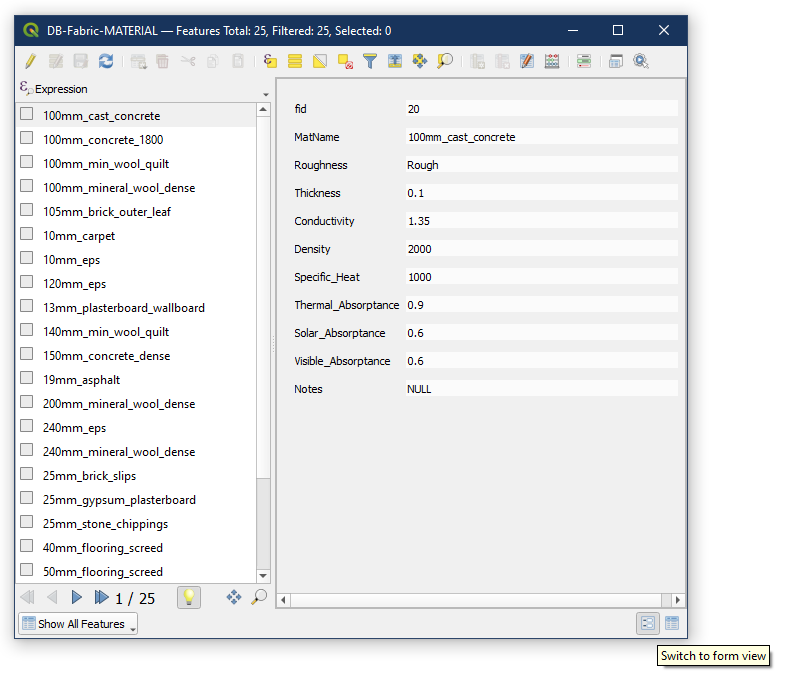
\includegraphics[width=12cm]{Figures/databaselayer2.png}
    \caption{The same "\texttt{MATERIAL}" database layer, in Form View.}
    \label{fig:db2}
\end{figure}

\subsubsection{Using constructions}
A set of default construction presets have been included with the plugin:
\begin{itemize}
    \item \texttt{const1}: Quincha wall with mud roof
    \item \texttt{const2}: Adobe wall with mud roof
    \item \texttt{const3}: Timber wall with corrugated metal roof
    \item \texttt{const4}: Brick wall with corrugated metal roof
    \item \texttt{const5}: Brick wall with concrete roof
\end{itemize}
To select one of these constructions for a given polygon, simply enter the name (e.g. \texttt{const3}) in the `constructions' field in the attribute table. \\

\textbf{Construction components} \\
Each construction is composed of separate elements which make up the construction. These are:
\begin{itemize}
    \item \texttt{constX\_wall}
    \item \texttt{constX\_roof}
    \item \texttt{constX\_ground\_floor}
    \item \texttt{constX\_ceiling}
    \item \texttt{constX\_ceiling\_inverse}\footnote{`ceiling\_inverse' is composed of the exact same layers as `ceiling' but in reverse order. If there is only one layer, it is identical to `ceiling'.}
\end{itemize}
where \texttt{X} is a unique number. The `\texttt{ceiling}' and `\texttt{ceiling\_inverse}' do not exist for Quincha/Timber constructions since these must not have more than one floor. The `Notes' field of the database layer provides information on each element. \\

The materials contained in the constructions can be found in the \texttt{MATERIAL} database. Some materials are shared amongst multiple constructions, so if you want to make a change which only affects one construction, you may have to duplicate materials. Remember to change the names to something unique and reference these in the relevant construction layer(s). \\

If you want to add a whole new construction preset, ensure that you add all of the elements above. Also ensure that you have spelled the names of the materials correctly. To learn how to make changes to the database, see Section~\ref{section:editingdb}.

\subsubsection{Mixed-use}
\label{section:mixeduse}
There are three options for floor use: `Dwell', `Commercial' and `Workshop'. This is entered in the `\texttt{FLOOR\_X:~use}' field in the attribute table. This will determine which database objects are selected for that particular floor. The database objects affected by this choice are:
\begin{itemize}
    \item People
    \item Lights
    \item Electric equipment
    \item Schedules
\end{itemize}
Each of the database layers above have unique entries for `Dwell', `Commercial' and `Workshop'. If the use field is not present, `Dwell' will be applied to all zones.

\subsubsection{Editing the database}
\label{section:editingdb}
Edit mode can be activated by selecting the pencil icon in the top-left corner (see Figures~\ref{fig:db1}\&\ref{fig:db2}). You can now make edits to any of the fields in the database. \textbf{When you have finished making changes, select the pencil icon again to turn off editing mode.} QGIS will ask if you would like to save these changes. If yes is selected, the changes will be saved to the \texttt{Simstock-Database.gpkg} file within your cwd. \\

Warning:
\begin{itemize}
    \item Do not change the database layer names
    \item Do not name any other layers ``\texttt{DB-...}''
    \item If you make edits, check for duplicates or misspellings -- these will cause errors during simulation.
\end{itemize}

\subsection{Running Simstock and the simulations}
After the input data is setup, Simstock can be run. This will take in all the information (geometry, attribute table, database) and Simstock will produce EnergyPlus models of the area. These model \texttt{idf} files will be output into the cwd. The plugin will then automatically launch the EnergyPlus simulations. The results will be loaded as a new layer in QGIS. The raw results will also be output into the cwd.

\subsubsection{Built islands}
The area is initially divided into `built islands'. A built island is defined as a group of buildings which are physically touching (excluding those which only share a single point). Each built island is given a unique reference number (\texttt{bi\_ref}). In the results layer, every polygon is given a \texttt{bi\_ref} to indicate which built island it belongs to. The \texttt{bi\_ref} can be used to locate the relevant \texttt{idf} file if necessary.

\subsubsection{Re-running}
There are two things to note before re-running the plugin:
\begin{itemize}
    \item The Simstock QGIS plugin will need to be reloaded (using the plugin reloader) before it can be run again.
    \item If you are editing the database between test cases, it is a good idea to make a copy of the previous database file (and give it a useful name) so that you can refer back to the setup when analysing the results.
\end{itemize}

\subsection{Results}
The results will appear as a new layer in QGIS. To save the layer, it must be converted from a temporary `scratch' layer into a permanent layer. This can be done by right-clicking on the layer and selecting `Make Permanent'. QGIS will then ask in what form to save it. It is possible to append this layer to an existing Geopackage if desired. \\

Note: Do not re-run Simstock on a results layer. It will not be able to populate result fields since they already exist. Instead, use the original layer which was used to produce the result layer.


\clearpage
\subsection{Implementing `retrofit' measures}
The following measures can be applied:
\begin{itemize}
    \item \textbf{Change building fabric} -- via the database layers
    \item \textbf{Change ventilation rates} -- via the attribute table
    \item \textbf{Add shading overhang to windows} -- via the attribute table
    \item \textbf{Simulate heating and cooling} -- see below
\end{itemize}

\subsubsection{Toggling heating and cooling loads}
\label{section:heatingcoolingtoggle}
You can decide whether to turn on/off the heating and cooling setpoints before running the simulations. The database layer named `\texttt{DB-HeatingCooling-OnOff}' contains a TRUE/FALSE field which can be edited.
\begin{itemize}
    \item \textbf{FALSE} (default) -- Heating and cooling are turned off and any resulting electricity demand is solely due to the lighting and electric equipment.
    \item \textbf{TRUE} -- Heating and cooling are turned on. The setpoint schedules are sourced from the \\
    `\texttt{DB-Schedules-SCHEDULE\_COMPACT}' layer.
\end{itemize}

The name of the outputted results layer states whether heating + cooling were activated for that specific simulation.

\section{Contact \& feedback}
We hope you have a smooth and enjoyable experience using the Simstock QGIS plugin! If you have any feedback, issues or other comments, please email me at: \texttt{shyam.amrith.14@ucl.ac.uk}

\clearpage
\appendix
\section{Notes for teachers and developers}
\subsection{Python errors}
If a Python error occurs, a yellow notification appears in QGIS. The error can be viewed by clicking `Stack Trace'.

\subsection{EnergyPlus errors}
If EnergyPlus failed to complete the simulation, the plugin will halt and a Python error will be raised to inform of this. Within the user's specified cwd, a folder will exist called `\texttt{idf\_files}'. In here, there will be sub-directories for each built island simulation within which the EnergyPlus \texttt{.err} files can be found. \\

In the absence of the result layer, each polygon can be matched to its \texttt{bi\_ref} (and therefore its idf file) by checking the intermediate \texttt{csv} file created. This will be located in the plugin directory and named \texttt{sa\_preprocessed.csv}.

\subsection{Config file}
Certain settings can be edited in the \texttt{config.json} file if necessary. This can be found in the plugin directory. \\

Currently editable fields and what they represent:
\begin{itemize}
    \item \textbf{Low temperature threshold}: Number of hours \textit{below} this operative temperature threshold will be reported in the results (default: $18^{\circ}$C).
    \item \textbf{High temperature threshold}: Number of hours \textit{above} this operative temperature threshold will be reported in the results (default: $28^{\circ}$C).
    \item \textbf{CRS}: Coordinate reference system for the current project (default: `\texttt{epsg:32718}').
    \item \textbf{epw}: Name of the weather file used for simulations. The specified file must be located at the base of the plugin directory (default: \texttt{PER\_LMA\_Lima-Chavez.Intl.AP.846280\_TMYx.2007-2021.epw}).
    \item \textbf{Cooling COP}: The coefficient of performance (COP) of the cooling system (default: 2.5).
    \item \textbf{Grid factor -- kgCO2/kWh}: The carbon intensity of the electricity grid (default: 0.234 kgCO2/kWh).
    \item \textbf{Electricity cost -- currency/kWh}: The cost of electricity per kilowatt hour (default: 0.15 currency/kWh).
    \item \textbf{Currency}: The symbol of the currency used in the above electricity cost. This symbol will be inserted into the results table (default: \$).
\end{itemize}

\subsection{File caching}
Note that if any changes are made to any of the plugin files, it is highly recommended to restart QGIS instead of simply reloading the plugin as some files can be cached.

\subsection{Alternative UI for high-dpi displays}
On some high-dpi displays, the plugin may not render correctly. If this is a problem, the UI can be switched to a scale-able version. Note that this new UI, whilst scale-able, can also suffer from distortions. \\

To switch UI, rename the following file:
\begin{center}
`\texttt{Simstock\_QGIS\_dialog\_base\_highdpi.ui}' \hspace{2mm} $\rightarrow$ \hspace{2mm} `\texttt{Simstock\_QGIS\_dialog\_base.ui}'.
\end{center}
Keep the old \texttt{.ui} file in case it is necessary to revert back.

\section{Credit}
EnergyPlus v8.9 is packaged as part of the Simstock QGIS Plugin. The official EnergyPlus website can be found here: \url{https://energyplus.net/} \\

Eppy is packaged as part of the Simstock QGIS Plugin. The project's homepage on PyPI can be found here: \url{https://pypi.org/project/eppy/}

%\fi

\iffalse
\section{To add}
\begin{itemize}
    \item Understanding the interface
    \item Plugin reloader
    \item Make Python console bit more prominent
    \item Types to use in each field
    \item Built islands (what they are, ref system, things to watch out for (i.e. name will change if more buildings are lassoed to the same BI)
    \item Add fields fn (and that it must be run after entering nofloors)
\end{itemize}
\fi

\end{document}
